
\section{Agentic Replacement: Agent(s) as Recommender}\label{sec:agent_as_recommender}

\subsection{Definition and Scope}\label{subsec:agent_rec_def}

{The paradigm \emph{agent as recommender} refers to systems in which an intelligent agent directly assumes the role of the recommender rather than merely supporting a conventional recommendation pipeline. In such systems, the agent is the end-to-end decision maker that (i) interprets user intent, (ii) maintains user state over time, (iii) selects and executes actions that may include tool invocation and external information gathering, and (iv) produces the final recommendation and natural-language response. The distinguishing feature is \emph{decision authority}: classical recommendation models, if present, are invoked as tools rather than acting as the primary controller \cite{huang2024interecagent,wang2024recmind}.} 


{
To systematize the diverse methodologies in agent as recommender, we categorize existing works into two primary architectural paradigms: \textbf{Single-Agent} and \textbf{Multi-Agent}. While both paradigms share the fundamental components of agents (such as Profile, Memory, Tool-Using, Workflow, and Optimization), they diverge fundamentally in how these components are orchestrated and how decision-making authority is distributed.
}


\textbf{Single-Agent based Recommender} functions as a centralized, monolithic decision-maker. In this paradigm, a single agent acts as the unified ``brain,'' responsible for the entire lifecycle of the recommendation process—from interpreting user intent and managing internal memory to invoking tools and generating the final response. The core challenge here lies in enhancing the individual agent's capabilities to handle complex reasoning chains without losing context or coherence. As detailed in \S~\ref{subsec:agent_rec_components}, our discussion focuses on how individual modules (e.g., Profile, Memory) are internalized within a single entity to achieve proactivity and adaptivity.

\textbf{Multi-Agent based Recommender}, in contrast, operates as a decentralized collaborative ecosystem. Here, the recommendation task is decomposed into sub-problems assigned to specialized agents (e.g., a Planner, a Critic, or a Domain Expert). The system's intelligence emerges not from a single model's depth but from the interaction between agents. This paradigm addresses the limitations of single-agent contexts by distributing cognitive load and introducing mechanisms like debate and role-playing. Consequently, in \S~\ref{subsec:agent_rec_multi}, our focus shifts from internal modules to inter-agent dynamics, specifically emphasizing \textit{Communication} protocols and collective \textit{Optimization}.

This taxonomy allows us to dissect how the five core components evolve: roughly speaking, what manifests as an internal \textit{Workflow} in a single agent often scales into a \textit{Communication} protocol in a multi-agent system; similarly, internal \textit{Self-Reflection} evolves into peer-to-peer \textit{Feedback}. 
{
In the following, we first elaborate on \textit{single-agent based recommender}, discussing how the five core components are internalized within a single agent to achieve proactivity and adaptivity for recommendation (\S \ref{subsec:agent_rec_components}). 
Then, we shift from internal modules to inter-agent dynamics and focus on \textit{Multi-Agent based Recommender} (\S \ref{subsec:agent_rec_multi}), specifically emphasizing \textit{Communication} protocols and collective \textit{Optimization}. 
}



\subsection{Single-Agent Recommenders (LoA L4)}\label{subsec:agent_rec_components}

\textbf{Modeling recommender as a single agent substantially upgrades their high-level capabilities beyond what traditional model-centric pipelines can offer.} 
1) As a unified decision-making entity, a single agent enables \textit{proactivity}, transitioning the system from purely reactive responses to actively inferring needs, initiating clarifications, and planning ahead within a session. 2) It also enhances \textit{context awareness} by maintaining a coherent internal state: while the underlying model is constrained by a finite context window, the agent can leverage explicit memory or state tracking to preserve user preferences and interaction history across turns. 
3) Moreover, the single-agent paradigm improves \textit{interaction flexibility}, supporting multi-turn, natural-language preference elicitation and iterative refinement rather than single-shot prediction. 
4) Finally, a single agent introduces \textit{stronger adaptivity}: it can continuously update its internal beliefs, adjust its recommendation strategy based on ongoing feedback, and self-correct within a session, instead of acting as a static mapping from input to output. Together, these improvements make the single-agent recommender more conversational, contextually grounded, and behaviorally adaptive than traditional recommender systems.


{To systematize the literature, we follow a reusable decomposition into five components: profile (\S \ref{subsubsec:agent_rec_profile}), memory (\S \ref{subsubsec:agent_rec_memory}), tool-using (\S \ref{subsubsec:agent_rec_tools}), workflow (\S \ref{subsubsec:agent_rec_workflow}), and optimization (\S \ref{subsubsec:agent_rec_optimization}). This decomposition is practical because it enables comparison between systems that differ in task setting (\eg conversational versus sequential recommendation) but share common control-loop structures.}

\subsubsection{\textbf{Profile: Persistent Preference and Constraint Modeling}}\label{subsubsec:agent_rec_profile}

{The \emph{profile} is a persistent representation capturing long-term preferences, constraints, and relatively stable aspects of user intent. Unlike classical recommenders where profiles are often implicit (encoded in latent embeddings), agentic recommenders frequently maintain explicit textual or structured profiles to support interpretability and controllability \cite{huang2024interecagent,tang2025interactive}. Profiles can be constructed by summarizing interaction histories into preference statements, maintaining structured constraint lists (budget, time, category exclusions), or extracting higher-level values that explain the user’s choices.}


{
In agentic recommender systems, the profile serves as the foundation for modeling both users as autonomous entities with distinct goals, preferences, and behavioral patterns.
For instance, in InteRecAgent~\cite{huang2024interecagent}, the profile module maintains a structured user representation comprising three facets (i.e., like, dislike, and expect) which are dynamically synthesized by the LLM from conversational history to capture both long-term preferences and short-term intentions for tool invocation.
Instruct$^2$Agent~\cite{xu2025iagent}  maintains an instruction-aware profile updated with round-wise user feedback and a dynamic extractor that derives task-specific preferences under current instructions, enabling per-user optimization decoupled from other users.
}

\subsubsection{\textbf{Memory: Working, Episodic, and Semantic State}}\label{subsubsec:agent_rec_memory}
{Memory is a core component that supports contextual reasoning and provides grounding evidence that constrains the agent’s outputs. A useful abstraction distinguishes: (i) \textbf{\textit{working memory}} (short-term conversational context), (ii) \emph{\textbf{episodic memory}} (retrievable records of prior interactions and feedback), and (iii) \emph{\textbf{semantic memory}} (abstracted preference facts and world knowledge) \cite{wang2024recmind,liu2025agentcf++}.} 
Memory can also take different forms, including \textbf{textual} (explicit) representations, \textbf{parametric} (implicit) representations, or none.



\begin{table}[!t]
\caption{Taxonomy of memory mechanisms and representative works in agentic recommender systems.}
\label{tab:memory}
\small
\setlength{\tabcolsep}{4pt}
\begin{tabularx}{\columnwidth}{p{0.18\columnwidth} X p{0.28\columnwidth}}
\toprule
\textbf{Memory Type} & \textbf{Representative Work} & \textbf{High-level Capabilities} \\
\midrule
\textbf{Working Memory} 
& InteRecAgent~\cite{huang2024interecagent}, ToolRec~\cite{zhao2024toolrec}, AgentRecBench~\cite{shang2025agentrecbench}, InstructAgent~\cite{xu2025iagent}, AgentDR~\cite{yang2025agentdr}, RuleAgent~\cite{wang2025ruleagent}, PUMA~\cite{cai2025large}, VibeMus~\cite{guo2025vibemus}, Sunnie~\cite{wu2024sunnie}
& \multirow{3}{=}{\newline\textbf{Context Awareness:} Memory\newline
\textbf{Interaction Flexibility:} Strengthen multi-turn interaction\newline
\textbf{Adaptivity:} Continuous evolving} \\
\cmidrule{1-2}
\textbf{Episodic Memory} 
& PUMA~\cite{cai2025large}
& \\
\cmidrule{1-2}
\textbf{Semantic Memory} 
& RecMind~\cite{wang2024recmind}, AFL~\cite{cai2025agentic}, RecAI~\cite{lian2024recai}, InstructAgent~\cite{xu2025iagent}, AgentDR~\cite{yang2025agentdr}, MemRec~\cite{chen2026memrec}
& \\
\bottomrule
\end{tabularx}
\end{table}

{
We summarize the three types of memory and how it achieves different agentic capabilities in Table~\ref{tab:memory}, while we give some concrete examples as follows. 
In InteRecAgent~\cite{huang2024interecagent}, the memory module is realized as a Candidate Bus, which maintains current item candidates separately from the prompt by combining a data bus—initialized at each conversation turn with all items or user-specified candidates and updated after each tool execution—and a tracker that logs each tool’s input, output, and execution status, enabling sequential streaming of candidates through multiple tools and supporting the reflection mechanism for judgment.
RecMind~\cite{wang2024recmind} defines a Memory component split into: Personalized Memory, which stores individual user data (e.g., their ratings or reviews), and World Knowledge, which stores item metadata (domain‑specific) and real‑time information via web search.  
BiLLP~\cite{shi2024planner} designed dedicated working memory modules for each of its key components (e.g., actor, critic, and planner) to store past experiences, with memory updated after each step.
The memory of \cite{yu2025intelligent_agent} selectively stores relevant item features, user reviews, and interaction history to support accurate and personalized recommendations continuously.
}





{
\subsubsection{\textbf{Tool-Using: Expanding the Action Space.}}\label{subsubsec:agent_rec_tools}
A key characteristic of agentic systems is their ability to augment reasoning through external tools, enabling agents to dynamically interact with APIs, databases, search engines, or specialized modules to enhance their recommendation capabilities. We categorize the tools employed by existing agents into four main types:
(1) \textbf{RecTools}: Tools for retrieval, ranking, or classical recommender system engines, which form the core mechanism for filtering relevant candidates and predicting user preferences;
(2) \textbf{External knowledge}: Tools that access knowledge bases or search engines beyond the recommendation system, supporting responses to user queries that require real-time or external information~\cite{guo2024knowledge};
(3)
\textbf{Attribute tools}: Schema-aware or faceted filters for attribute-oriented retrieval, allowing fine-grained control over item selection;
(4)
\textbf{Multimodal tools}: Tools designed to handle additional modalities such as images, audio, or code, extending the agent’s capability beyond textual information.}

{
For instance, in InteRecAgent~\cite{huang2024interecagent}, retrieval and ranking tools serve as the core recommendation engines by identifying relevant candidates and estimating user preferences, while information query tools allow the agent to access external knowledge bases or databases via SQL and search engines to answer user inquiries beyond standard recommendation tasks.
RecMind~\cite{wang2024recmind} mainly integrates three types of tools to access and process external knowledge: a Database Tool that converts natural language queries into SQL to retrieve in-domain knowledge such as user reviews or item metadata; a Web Search Tool for fetching real-time information from the internet as part of world knowledge; and a Text Summarization Tool to process and condense the retrieved information.
In the multi-agent collaboration framework proposed by MACRec~\cite{macrec}, the Analyst is granted access to two tools to assist in analysis: an information database to get the user profile and item attributes and an interaction retriever to get the user/item interaction history.
ToolRec~\cite{zhao2024toolrec} introduces attribute-oriented retrieval and ranking tools: retrieval tools first return candidate items based on specified attribute patterns and size constraints, while ranking tools use LLMs with instruction templates to order these candidates according to user history and attribute relevance, effectively capturing users’ latent intent without training separate models for each attribute.
\cite{shi2024planner} define a Category Analysis Tool which can identify a list of categories associated with each legal action and conduct a statistical analysis on the user’s
viewing history.
AgentDR~\cite{yang2025agentdr} bridges LLM reasoning with scalable rec tools by delegating full-catalog ranking to traditional recommenders while using the agent to integrate multiple model outputs (personalized tool suitability) and inject commonsense relational reasoning over substitutes/complements grounded in the user’s history—mitigating hallucination and keeping the system scalable.
}






\begin{table}[!t]
\caption{Taxonomy of workflow controllers in agentic recommendation systems.}
\label{tab:workflow_controllers}
\vspace{-8pt}
\small
\setlength{\tabcolsep}{4pt}
\begin{tabularx}{\columnwidth}{p{0.18\columnwidth} X p{0.28\columnwidth}}
\toprule
\textbf{Workflow Type} & \textbf{Representative Work} & \textbf{High-level capabilities} \\
\midrule
\textbf{ReAct} 
& RecMind~\cite{wang2024recmind}, ToolRec~\cite{zhao2024toolrec}, AgentRecBench~\cite{shang2025agentrecbench}, PUMA~\cite{cai2025large}, WeMusic-Agent\cite{bi2025wemusic}
& \multirow{3}{=}{\newline \textbf{Proactivity}: proactive \& reactive,\newline \newline
\textbf{Interaction Flexibility}: Multi-turn,\newline \newline
\textbf{Adaptivity}: continuous evolving} \\
\cmidrule{1-2}
\textbf{Plan-then-Execute} 
& InteRecAgent~\cite{huang2024interecagent}, AFL~\cite{cai2025agentic}, RecAI~\cite{lian2024recai}, AgentRecBench~\cite{shang2025agentrecbench}, InstructAgent~\cite{xu2025iagent}, CogRec~\cite{hu2025cogrec}, ScienceDB AI~\cite{long2026sciencedb}, AMEM4Rec~\cite{nguyen2026amem4rec}
& \\
\cmidrule{1-2}
\textbf{Reflex}
& AgentRecBench~\cite{shang2025agentrecbench}, AgentDR~\cite{yang2025agentdr}, RuleAgent~\cite{wang2025ruleagent}
& \\
\bottomrule
\end{tabularx}
\end{table} 

\subsubsection{\textbf{Workflow Controllers: From Reasoning--Acting to Reflection}}\label{subsubsec:agent_rec_workflow}


\begin{figure}[t]
\setlength{\abovecaptionskip}{-0.0cm}  
\setlength{\belowcaptionskip}{-0.0cm} 
    \centering
    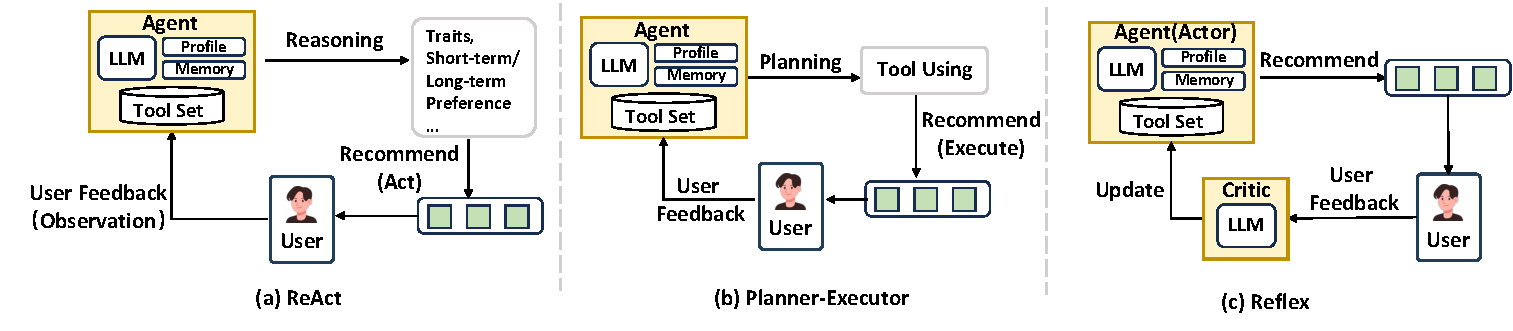
\includegraphics[width=1\linewidth]{figures/workflow.pdf}
    \caption{Three paradigms of workflows of single-agent recommenders.}
    \label{fig:workflow}
    % \vspace{-8pt}
\end{figure}


{The workflow controller specifies how the agent sequences reasoning steps and actions. As illustrated in Figure~\ref{fig:workflow}, three recurring patterns are prominent.}
Table~\ref{tab:workflow_controllers} summarizes these workflow paradigms, along with representative methods and their associated high-level capabilities. 
Overall, ReAct emphasizes flexible interaction and incremental reasoning, Plan-then-Execute improves controllability and structured decision-making, while Reflex enables continuous policy refinement through self-evaluation. 
These complementary designs collectively support key agentic capabilities, including proactivity, multi-turn interaction flexibility, and adaptive evolution.



\noindent$\bullet\quad$\textbf{ReAct (interleaved reasoning and acting).}
{In this pattern, the agent alternates between intermediate reasoning and tool invocation, supporting incremental refinement of candidates and constraints \cite{yao2022react}. This is effective for open-ended requests but can compound errors if early tool calls are misguided.} 
{
A large portion of existing work lies in this workflow. MoRE~\cite{more} introduces a reflection-based framework for sequential recommendation, where an LLM dynamically selects and combines multiple reflectors to iteratively reconsider and correct its recommendation decisions, mitigating biases and instability caused by a single reasoning path. DRDT~\cite{drdt} uses dynamic reflection with divergent thinking within a retriever–reranker framework to iteratively probe, critique, and tailor LLM reasoning to better model sequential user preferences over time.
R4ec~\cite{gu2025r} establishes a reasoning–reflection–refinement loop where an actor model proposes recommendations and a reflection model evaluates and feeds back corrections, enabling deliberate System-2-like thinking to improve recommendation accuracy. Re2LLM~\cite{re2llm} guides LLMs to self-reflect on recommendation errors to build a hint knowledge base and trains a lightweight agent to select useful hints that correct reasoning, resulting in more accurate session-based recommendations without fine-tuning the LLM. SRLF~\cite{srlf} introduces a set-wise reflective learning framework that uses an LLM agent to assess entire candidate item sets, detect mismatches with user feedback, and iteratively refine both user preferences and item semantics through a closed-loop reflection process, capturing richer inter-item relationships for better sequential recommendation. 
}


\noindent$\bullet\quad$\textbf{Plan-then-Execute.}
{Here, a planner decomposes the user request into subgoals (\eg constraint inference, candidate retrieval, verification) and an executor carries out tool calls under this plan. This improves controllability because plans can be inspected and constrained \cite{huang2024interecagent,yu2025thought}.} 
For example, InteRecAgent~\cite{huang2024interecagent} adopts a plan-first execution workflow consisting of two stages: in the first stage, the LLM generates a complete tool-utilizing plan based on the user query; in the second stage, the system executes each operation sequentially according to the plan, without invoking the LLM at every step. 
RecMind~\cite{wang2024recmind} introduces a Self-Inspiring (SI) planning method that leverages all previously explored reasoning branches to generate each step, enabling more comprehensive and multi-perspective reasoning for recommendation tasks than traditional single-path approaches like CoT~\cite{wei2022cot} and ToT~\cite{yao2023tot}. 
Instruct$^2$Agent~\cite{xu2025iagent} follows plan-then-execute (parser $\rightarrow$ knowledge/tool use $\rightarrow$ reranker) with a reflex-style self-reflection that regenerates constrained lists when inconsistencies are detected.



\noindent$\bullet\quad${
\textbf{Reflex}: Self‑critique loop or judge–checker pattern~\cite{wu2025starec,wu2025personalized}.
BiLLP~\citet{shi2024planner}  
follow the actor-critic framework and initialize the actor and critic as using LLM, 
to provide personalized recommendations, where Critic assesses the user’s
current satisfaction level (action advantage value) and updates
the policy of Actor to enhance personalized recommendations.
T-PRA~\cite{wang2025t-pra} adopts an actor–critic framework to balance the trade-off between user satisfaction and user
interest exploration in proactive conversational recommendation.
AgentDR~\cite{yang2025agentdr}follows plan-then-execute with a reflex-style check: the agent plans which base recommenders to consult, aggregates their candidates, reasons about item-item substitutes/complements, and re-scores candidates before output—acting as a controller atop conventional rankers rather than a monolithic generator.
}



\subsubsection{\textbf{Optimization and Adaptation}}\label{subsubsec:agent_rec_optimization}



{
To continuously enhance the decision-making capabilities, recommendation agents must perform optimization over time—refining their internal policies and strategies through iterative learning.
Such optimization processes can be broadly categorized into two complementary paradigms:
(1) \textbf{Self reflection}, where the agent evaluates and improves upon its own reasoning and recommendations; and
(2) \textbf{Feedback reflection}, where the agent adapts based on external signals from the environment or user feedback.
Together, these mechanisms enable agents to move beyond static policy learning toward agentic optimization, characterized by proactive self-improvement and adaptive alignment with long-term user goals.
}

\begin{figure}[t]
\setlength{\abovecaptionskip}{-0.0cm}  
\setlength{\belowcaptionskip}{-0.0cm} 
    \centering
    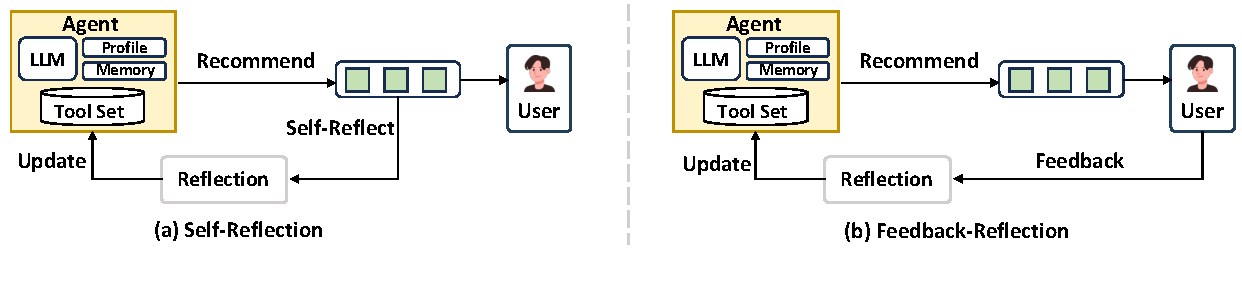
\includegraphics[width=0.8\linewidth]{figures/optimization.pdf}
    \caption{Two paradigms of optimization in single-agent recommenders.}
    \label{fig:optimization}
    % \vspace{-10pt}
\end{figure}

{
\textbf{Self-Reflection:}
Self-reflection focuses on internal critique and self-improvement loops, where the agent evaluates the quality of its own decisions and refines its policy accordingly.
For instance, T-PRA~\cite{wang2025t-pra} introduces a critic module that generates structured feedback on recommendation outcomes. This feedback is then leveraged via Direct Preference Optimization (DPO) to jointly refine both the actor and advisor components, improving alignment with long-term proactive recommendation objectives.

\textbf{Feedback-Reflection:} In contrast, feedback-reflection leverages external signals from user interaction or environment feedback to guide optimization.
ECPO~\cite{feng2025expectation} exemplifies this paradigm by modeling user expectations and confirmations at each conversational turn. It identifies sources of user dissatisfaction and performs fine-grained, turn-level preference updates. This design improves multi-turn interaction quality while avoiding the high sampling cost associated with prior methods such as MTPO.
}



\subsection{Multi-Agent Recommenders (LoA L5)}\label{subsec:agent_rec_multi}



\textbf{Beyond the capabilities enabled by a single agent, multi-agent recommenders introduce an additional layer of enhancement by distributing decision-making across multiple specialized agents.} 
1) In terms of proactivity, multi-agent systems move from individual proactive reasoning to \textit{collective proactivity}, where different agents—such as planners, critics, retrievers, and preference elicitors—jointly anticipate user needs and cross-check each other’s actions, leading to more reliable proactive behaviors than a single agent. 
2) For context awareness, multi-agent architectures alleviate the limitations of a single agent’s context window by allowing each agent to maintain its own perspective or memory, resulting in distributed memory that captures user intent, item evidence, and environmental constraints more completely. 
3) Regarding interaction flexibility, multi-agent setups transform single-agent multi-turn interaction into multi-party collaborative interaction: agents can debate, critique, refine, or negotiate with one another before presenting results to the user, enabling richer reasoning patterns than any single agent can achieve. 
4) Finally, in terms of adaptivity, multi-agent systems support continuous evolving behavior not only through user feedback but also through internal self-correction loops—where agents iteratively refine each other’s outputs—making the system more adaptive and stable compared to a single adaptive policy. 
Overall, while single-agent systems enhance recommendation along the four dimensions within one coherent policy, multi-agent systems amplify these capabilities through structured cooperation, role specialization, and self-consistency mechanisms.

\subsubsection{\textbf{Roles and Coordination Protocols}}\label{subsubsec:agent_rec_coordination}
Common role sets include manager/planner agents, retrievers, rankers, analyzers, critics, verifiers, and safety monitors. Coordination protocols vary: manager--worker decomposition \cite{wang2024macrec, xia2026multi, zhang2026llms,nie2024hybrid,portugal2024agentic,agarwal2024multistage}, debate--judge selection \cite{fang2024multi,ma2025agentrec}, role-based trustworthy conversational protocols \cite{hui2025matcha}, and negotiation-based approaches for multi-stakeholder recommendation \cite{banerjee2025collab, dixit2026pcn}. Hierarchical agent structures are also common in route and itinerary recommendation, where feasibility constraints naturally require staged reasoning and verification.

\subsubsection{\textbf{Communication}} Communication is a key mechanism enabling collaboration and coordination in multi-agent recommendation systems.
By exchanging information about user context, preferences, and reasoning outcomes, agents can jointly construct more accurate and consistent recommendations.
Such inter-agent communication fosters cooperative behaviors, mitigates information asymmetry, and supports the emergence of specialized agent roles for complex recommendation tasks.
MacRec~\cite{macrec} introduces a multi-agent collaboration framework, including the Manager, User/Item Analyst, Reflector, Searcher, and Task Interpreter, to enhance recommendation tasks.
MAS4POI~\cite{wu2025mas4poi} is a multi-agent framework (comprising agents such as DataAgent, Manager, Analyst, and Navigator) that collaboratively produces next point-of-interest (POI) recommendations. In each task, one or more agents are selected to perform the corresponding operation, and all agents are coordinated and their information aggregated through the manager agent.
MACRS~\cite{fang2024multi} decomposes the Conversational Recommender System (CRS) workflow into four LLM-based agents that plan dialogue acts, independently generate candidate responses, and then select a final response via a judge module. Beyond the policy side, MACRS also provides a more realistic user simulator by masking the target item with a keyword-level profile to reduce direct leakage and overly explicit hints.
In ARAG~\cite{maragheh2025arag}, agents communicate via staged hand-offs rather than free-form chat: understanding $\rightarrow$ alignment-scoring $\rightarrow$ evidence compression $\rightarrow$ ranking. This act-structured passing stabilizes dialogue flow and makes decisions diagnosable.
In RecBot~\cite{tang2025interactive}, communication between the Parser and Planner agents follows a structured hand-off protocol, where the Parser conveys normalized user intents to the Planner through explicit JSON-style messages, ensuring transparent coordination and preventing semantic drift during multi-turn command execution.
In Collab-REC~\cite{banerjee2025collab} , communication proceeds via moderated rounds: agents submit act-conditioned proposals; the moderator feeds back rejections and penalties (e.g., repeated or spurious cities) and requests revisions, yielding negotiated consensus rather than free-form chat.
TAIRA~\cite{yu2025thought} coordinates a Manager–Executors pipeline via structured hand-offs: the Manager selects a thought pattern, decomposes the user request into sub-tasks, and dispatches them to specialized Executors, who return evidence and partial results for aggregation—reducing semantic drift compared with free-form multi-agent chat.
In MATCHA~\cite{hui2025matcha}, inter-agent communication follows a structured role-based protocol, where the intent agent passes normalized user goals to the generator and ranker, and downstream explanation and safeguard agents exchange rationale and risk annotations to ensure coherent, transparent, and trustworthy collaboration.


\subsubsection{\textbf{Optimization}}\label{subsubsec:multi-agent-optimization}
Optimization in multi-agent recommendation systems focuses on improving collective decision quality without relying on gradient-based parameter updates.
Through mechanisms such as structured coordination, negotiation, and self-distillation, agents can iteratively refine their reasoning and cooperation strategies~\cite{acharya2026group, li2026recnet, wu2026internalizing, wang2026self, wang2026momorec, zhu2025llm_based_conv}.
Rather than relying on gradient-based updates, MACRS~\cite{fang2024multi} mainly optimizes the decision quality through structured coordination (parallel candidate generation followed by selection) and by adopting a more realistic user-simulation protocol.
ARAG~\cite{maragheh2025arag} optimizes recommendation quality by coordinating agents for consistency-aware evidence refinement, enabling the system to iteratively filter irrelevant retrievals and enhance ranking accuracy without retraining the backbone LLM.
RecBot~\cite{tang2025interactive} optimizes its dual-agent policy through simulation-driven distillation, where high-fidelity trajectories from a teacher model (e.g., GPT-4.1) are distilled into a lightweight student agent, enabling efficient online deployment while preserving reasoning and planning competence.
Collab-REC~\cite{banerjee2025collab} optimizes decision quality without fine-tuning LLMs by combining multi-round negotiation with a penalty-aware scoring function that rewards agent success while penalizing repetition and hallucinated entries—explicitly steering the system toward balanced, diverse lists across stakeholders.
TAIRA~\cite{yu2025thought} optimizes agent behavior through thought-pattern distillation, a self-improving process that abstracts successful reasoning traces into reusable planning templates, enabling more consistent task decomposition and tool use without retraining the underlying LLM.



\subsection{Summary}\label{subsec:agent_rec_summary}

Agent-as-recommender systems represent the most direct realization of autonomy in recommendation: the agent becomes the controller and the decision maker. The literature indicates a progression from single-agent interactive controllers, to tool-learning and reflective workflows, and finally to multi-agent orchestration for robustness, negotiation, and complex domains. 
From agentic augmentation (\ie agent-assisted recommender) to agentic replacement (\ie agent as recommender), recommender systems are more proactive, have stronger context awareness, are more flexible in interactions, and more adaptive (\cf \S \ref{subsec:agent_rec_components} and \S \ref{subsec:agent_rec_multi}).
